\problemname{GPS}
You, like so many other people, have probably used the Global Positioning Systems (GPS), but have wondered how it actually works.
GPS positioning is based on a set of satellites orbiting Earth.
All satellites have a synchronized internal clock\footnote{In practice the clocks are not completely synchronous -- because of general relativity. In this problem we assume that these effects do not exist.}.
They continuously transmit the value of their internal clock to the surface of Earth via radio waves.
A GPS receiver simultaneously\footnote{Another simplification.} collects measurements from some satellites which are in sight.
The time measurements $t_1,\dots,t_m$ collected at time $t$ are typically different, as each satellite has a different distance to the receiver.
Since we know the exact orbits of all satellites, we know exactly where each satellite was when it sent its signal.
Based on these positions and the distance, we can compute our position.
To compute a unique position, assuming that we are on the surface of the Earth, we need at least $3$~measurements from satellites.


Your task, however, is not to actually compute your own position, but to determine which signals you received from which satellites.
To be precise: you are given your geographical coordinates on Earth and a description of all orbits of satellites
and should now determine for every satellite 
\begin{itemize}
  \item whether a signal sent from the satellite at a certain time will reach you (which is the case if it does not pass through the Earth).
  \item if the signal does reach you, the time it took for the signal to travel from the satellite to your position.
\end{itemize}
Remember that radio waves travel in straight lines and at the speed of light, which we assume is $299\,792\,458$ meters per second.
We assume Earth to be a perfect sphere with a radius of $6\,371$km, and
that all GPS satellites are orbiting the Earth with a fixed speed on perfect circles whose centers are identical to the center of Earth.

\begin{figure}[h]
		\centering
		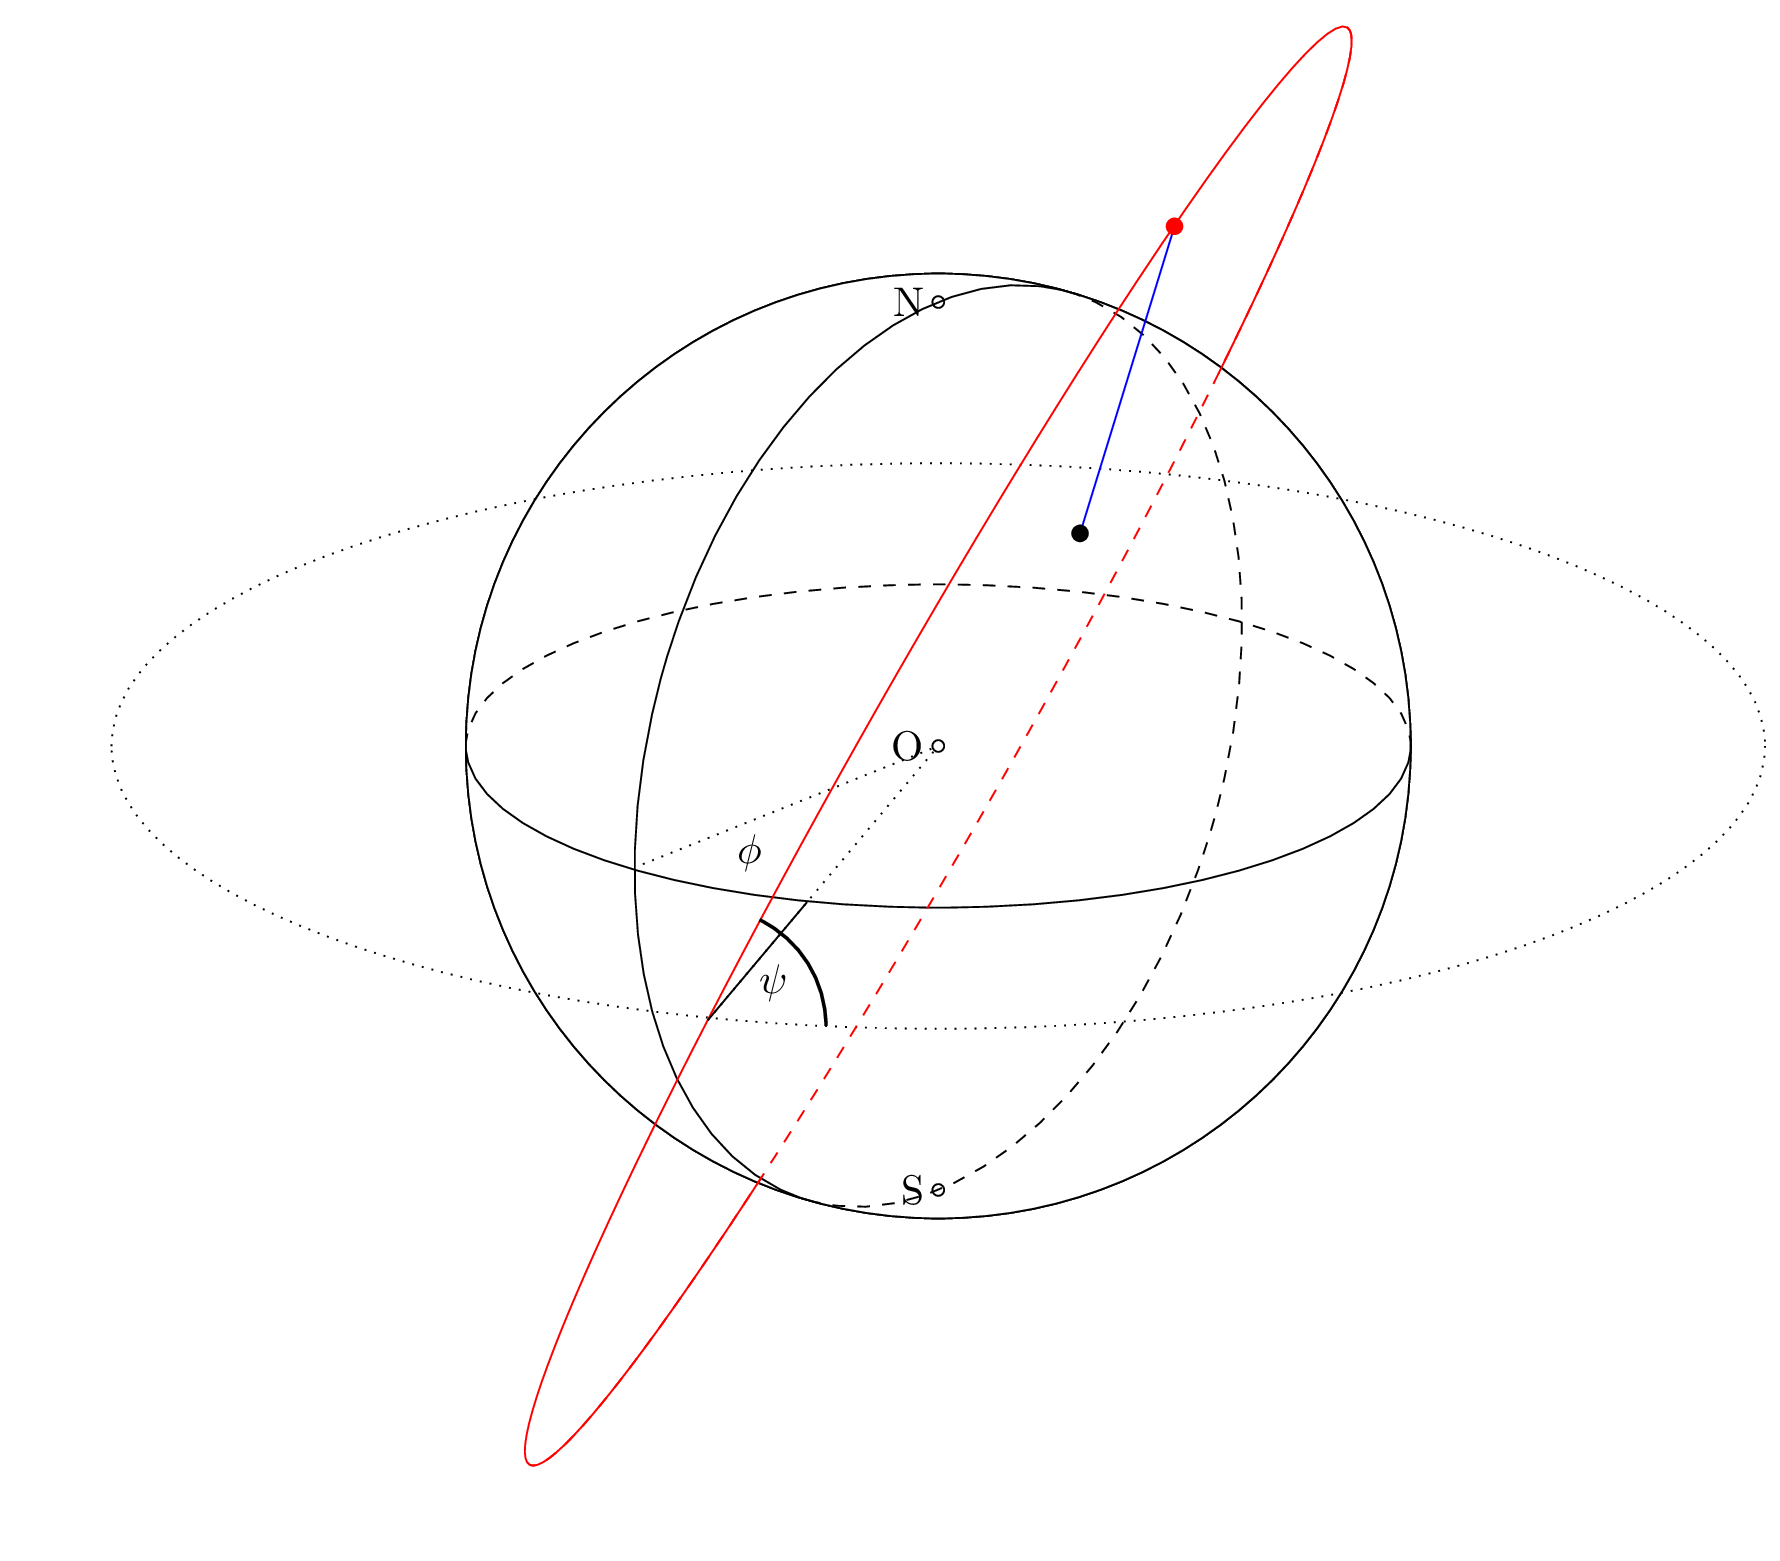
\includegraphics[width=.9\textwidth]{sphere.png}
		\caption{Schematic display of satellite coordinates.
				The satellite's orbit is shown in red, its actual position is the red dot.
        On Earth, the equator and the prime meridian are marked by lines.
				The dotted line is coplanar to the equator and has the same radius as the satellite's orbit.
				The angles $\phi$ and $\psi$ are described in the input section.
				The black dot is your position on Earth and you should compute the time necessary for
				the signal to travel the blue line.
		}
\end{figure}


\section*{Input}
The input consists of:
\begin{itemize}
  \item one line with an integer $s$ ($1 \le s \le 10^4$), the number of satellites;
  \item one line with two real numbers $\ell_o, \ell_a$, the longitude and latitude of your position;
  \item $s$ lines, each with four real numbers $\phi,\psi,r,x$ describing one of the satellites.
\end{itemize}

\noindent For the longitude $\ell_o\in[-180,180]$, positive values represent east and negative values west.\\
For the latitude $\ell_a\in[-90,90]$, positive values represent north and negative values south.

\noindent The format for the satellite descriptions is as follows:
\begin{itemize}
		\item $\phi \in [-180,180]$ -- the reference longitude at which the orbit intersects with the Earth's equator (each orbit intersects the equator (at least) twice).
				Positive longitude represents east, negative longitude represents west.
		\item $\psi \in [0,360]$ -- the angle between orbit and the Earth's eastbound equator when passing through the equator at longitude $\phi$.
				Values between $0$ and $180$ indicate northbound movement while values between $180$ and $360$ indicate southbound movement.
    			If the orbit is coplanar to the equator, the angle $\psi$ will be 0 or 180.
        \item $r \in [7\,000,10^6]$ -- the radius of the satellite's orbit in kilometers.
		\item $x \in [0,1)$ -- the fraction of the orbit the satellite had covered at the time when its signal was sent, starting from its intersection with the equator at $\phi$.
				%If the orbit is coplanar with the equator, this $x$ will count from longitude $0$.
\end{itemize}

\textbf{Note:}
All real numbers in the input are given with at most $3$ decimal places after the decimal point.
It is guaranteed that each satellite has a distance of at least $1$ meter from the tangent plane at your position (this means that you can safely use floating point arithmetic in your solution).

\section*{Output}
For every satellite, output \texttt{no signal} if a signal sent from that satellite does not reach you.
If the satellite's signal does reach you, output the time that the signal needs to travel from the satellite to your position, in seconds.
The time must be accurate up to a relative or absolute error (whichever is lower) of $10^{-7}$.

